\begin{figure}[h!]
	\centering
	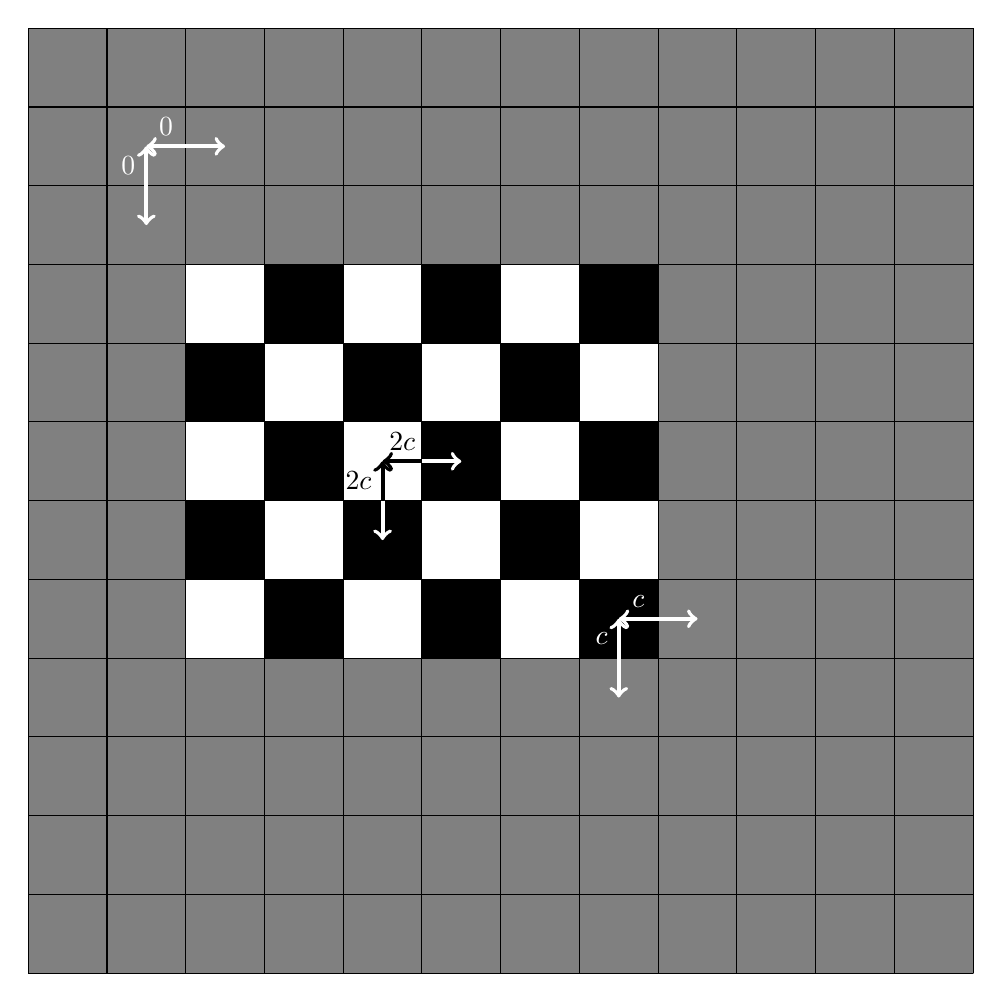
\begin{tikzpicture}
		\foreach \i in {-6, ..., 5}
			\foreach \j in {-6, ..., 5}
				\filldraw[gray] (\i, \j) rectangle + (1, 1);
		\foreach \i in {-4, ..., 1}
			\foreach \j in {-2, ..., 2}
			{
				\pgfmathparse{mod(\i+\j, 2) ? "black" : "white"}
				\edef\colour{\pgfmathresult}
				\filldraw[fill=\colour] (\i, \j) rectangle + (1, 1);
			}
		\draw[step=1] (-6, -6) grid (6, 6);
		\draw[<->, white, line width=0.5mm] (-4.5, 4.5) -- node[near start, above] {$0$} (-3.5, 4.5);
		\draw[<->, white, line width=0.5mm] (-4.5, 4.5) -- node[near start, left] {$0$} (-4.5, 3.5);
		\draw[<->, white, line width=0.5mm] (1.5, -1.5) -- node[near start, above] {$c$} (2.5, -1.5);
		\draw[<->, white, line width=0.5mm] (1.5, -1.5) -- node[near start, left] {$c$} (1.5, -2.5);
		\draw[<-, black, line width=0.5mm] (-1.5, 0.5) -- node[above] {$2c$} (-1, 0.5);
		\draw[->, white, line width=0.5mm] (-1, 0.5) -- (-0.5, 0.5);
		\draw[<-, black, line width=0.5mm] (-1.5, 0.5) -- node[left] {$2c$} (-1.5, 0);
		\draw[->, white, line width=0.5mm] (-1.5, 0) -- (-1.5, -0.5);
	\end{tikzpicture}
	\caption{Possible values of $\abs{V(i + 1, j) - V(i, j)}$ and $\abs{V(i, j + 1) - V(i, j)}$ as listed in Table \ref{table: discretederivativevalues}.}
	\label{fig: discretederivativevalues}
\end{figure}